\chapter{Отчёт по научно-исследовательской работе}
\label{cha:analysis}
\section{Постановка задачи}
В области $\Omega$ заданы уравнения равновесия \cite{Pisarenko1981}
\begin{equation}
%\sum\limits_{j=1}^{3} \frac{\partial\sigma_{ij}}{\partial x_j} = 0, i=\overline{1,3}.
%\frac{\partial\sigma_{ij}}{\partial x_j} = 0, i=\overline{1,3}.
%\bigtriangledown_j\sigma_{ij} = 0.%, i=\overline{1,3}.
\frac{\partial\sigma_{ij}}{\partial x_j} = 0.%, i=\overline{1,3}.
\label{F:F1}
\end{equation}
На границе $S=S_{1}\cup S_{2}$ заданы кинематические и силовые
краевые условия
\begin{equation}
\left.\mathbf{u}\right|_{S_{1}}=\mathbf{u}_{0}\left(t\right),
\label{F:F2}
\end{equation}
\begin{equation}
%\left.\sum\limits_{j=1}^{3}\sigma_{ij}n_j\right|_{S_{2}}=P_{i}\left(t\right),\:i=\overline{1,3},
\left.\sigma_{ij}n_j\right|_{S_{2}}=P_{i}\left(t,\,\mathbf{u}\right),% i=\overline{1,3},
\label{F:F3}
\end{equation}
\begin{equation}
\mathbf{P}\left(t,\,\mathbf{u}\right)=\mathbf{P}^t\left(t\right)+\mathbf{P}^c\left(t,\,\mathbf{u}\right),
\label{F:F_Contact_razlojenie}
\end{equation}
где $\mathbf{u}$ --- вектор перемещения, $\mathbf{n}$ --- внешняя единичная нормаль к поверхности $S_{2}$, $\mathbf{P}$ --- вектор поверхностных сил, $\mathbf{P}^t$ --- составляющая внешнего силового воздействия, $\mathbf{P}^c$ --- контактная составляющая на $S_c\subseteq S_2$.

На границе $S_{c}$ задаётся механический контакт с жёстким подвижным штампом геометрически нелинейными краевыми условиями Синьорини \cite{Kravchuk1994} 
\begin{equation}
\begin{cases}
\mathbf{P}^c\cdot\mathbf{n}\leq 0, \\
\mathbf{u}\cdot\mathbf{n}-g\leq 0, \\
\left(\mathbf{P}^c\cdot\mathbf{n}\right) \left(\mathbf{u}\cdot\mathbf{n}-g\right)=0, \\
\left( \mathbf{P}^c\cdot\mathbf{n}\right)\mathbf{n}=\mathbf{P}^c, \\
\end{cases}
\label{F:F_Contact_Signorini}
\end{equation}
где $\mathbf{n}\left(\mathbf{x},\,\mathbf{t}\right)$ --- внутренняя единичная нормаль в точке поверхности штампа, ближайшей к точке тела $\mathbf{x}$, $g\left(\mathbf{x},\,\mathbf{t}\right) $ --- расстояние от точки $\mathbf{x}$ до поверхности штампа (может принимать отрицательные значения в случае внедрения штампа).


Компоненты тензора малых деформаций Коши $\varepsilon$ связаны с перемещениями линейными геометрическими соотношениями
\begin{equation}
\varepsilon_{ij}=\frac{1}{2} \left(\frac{\partial u_{i}}{\partial x_{j}} + \frac{\partial u_{j}}{\partial x_{i}} \right).
\label{F:F4}
\end{equation}

Для изотропного тела тензор напряжений Коши $\sigma$ выражается через упругую составляющую $\varepsilon^{e}$ малой деформации Коши обобщенным законом Гука
\begin{equation}
%\sigma_{ij}=\sum\limits_{l=1}^{3} \sum\limits_{k=1}^{3} C_{ijkl}\varepsilon_{kl}^{e},
%\sigma_{ij}=C_{ijkl}\varepsilon_{kl}^{e},
\sigma=C:\varepsilon^{e},
\label{F:F_Hook}
\end{equation}
\begin{equation}
C_{ijkl}=\lambda\delta_{ij}\delta_{kl}+\mu\left(\delta_{ik}\delta_{jl}+\delta_{il}\delta_{jk}\right),
\label{F:F5}
\end{equation}
где $C$ --- тензор модулей упругости материала, $\lambda$, $\mu$ --- модули упругости Ламэ, $\delta$ --- символ Кронекера. Символом \textquotedblleft $:$\textquotedblright\ обозначено двойное скалярное произведение, т.е. $\left(C:\varepsilon\right)_{ij}\equiv C_{ijkl}\varepsilon_{kl}$.

Для связи напряжений и деформаций принимаются определяющие соотношения теории пластического течения \cite{Korobeynikov2000} с критерием текучести Мизеса:
\begin{equation}
d\varepsilon=d\varepsilon^{e} + d\varepsilon^{p},
\label{F:F_Flow1}
\end{equation}
\begin{equation}
\sigma_{y}=\Phi\left(q\right),
\label{F:F_Flow2}
\end{equation}
\begin{equation}
\begin{cases}
d\varepsilon_{ij}^{p}=\frac{\partial\tilde{\sigma}}{\partial\sigma_{ij}}d\lambda=\frac{\frac{3}{2}s_{ij}}{\tilde{\sigma}} d\lambda, \mbox{ если } \tilde{\sigma}=\sigma_{y} \mbox{ и } dW>0, \\
d\varepsilon_{ij}^{p}=0, \mbox{ если } \tilde{\sigma}<\sigma_{y} \mbox{ или } \tilde{\sigma}=\sigma_{y} \mbox{ и } dW\leq 0,
\end{cases}
\label{F:F_Flow3}
\end{equation}
где $d\lambda$ --- не известный множитель,
\begin{equation}
d\lambda=d\tilde{\varepsilon}^{p},
\label{F:F_FlowDef1}
\end{equation}
$\sigma_{y}$ --- предел текучести, $\Phi\left(q\right)$ --- функция, характеризующая поведение изотропно упрочняющегося материала (функцию $\Phi\left(q\right)$ можно построить по диаграмме одноосного растяжения, при котором $\tilde{\sigma}=\sigma$, $d\tilde{\varepsilon}^{p}=d\varepsilon^{p}$),
$d\varepsilon$, $d\varepsilon^{e}$, $d\varepsilon^{p}$ --- приращения полной, упругой и пластической деформаций соответственно, $\tilde{\sigma}\equiv\left(\frac{3}{2}s_{ij}s_{ij}\right)^{\frac{1}{2}}$ --- эквивалентное напряжение, $\tilde{\varepsilon}\equiv \left(\frac{2}{3}e_{ij}e_{ij}\right)^{\frac{1}{2}}$ --- эквивалентная деформация, $s_{ij}\equiv\sigma_{ij}-\delta_{ij}\frac{1}{3}\sigma_{kk}$ --- девиатор напряжений, $e_{ij}\equiv\varepsilon_{ij}-\delta_{ij}\frac{1}{3}\varepsilon_{kk}$ --- девиатор деформаций, $q$ --- параметр Одквиста,
\begin{equation}
q\equiv\int d\tilde{\varepsilon}^{p},
\label{F:F_FlowDef6}
\end{equation}
$dW$ --- девиаторная работа приращения деформаций,
\begin{equation}
dW\equiv s_{ij}d\varepsilon_{ij}.
\label{F:F_FlowDef7}
\end{equation}

В неизотермическом случае полная деформация представима в виде суммы объёмной деформации изотропного теплового расширения, пластической деформации и упругой деформации:
\begin{equation}
\varepsilon=\alpha T\delta+\varepsilon^p+C^{-1}:\sigma,
\end{equation}
где $T$ --- температура (относительно исходного состояния), $\alpha$ --- коэффициент линейного изотропного теплового расширения.

Рассмотрим приращение полной деформации $\Delta\varepsilon$ на шаге по времени \mbox{$t\longrightarrow t+\Delta t$}. Здесь и далее для переменных по умолчанию подразумевается момент времени $t+\Delta t$, а момент времени $t$ обозначается левым верхним индексом $(t)$; для областей и границ всегда подразумевается момент времени $t$ и обозначение времени опущено.
\begin{equation}
\begin{gathered}
\Delta\varepsilon={}^{(t+\Delta t)}\left(\alpha T\right)\delta-{}^{(t)}\left(\alpha T\right)\delta+\Delta\varepsilon^p+{}^{(t+\Delta t)}\left(C^{-1}:\sigma\right)-{}^{(t)}\left(C^{-1}:\sigma\right)=\\
=\underline{\left(\alpha\Delta T+T\Delta\alpha-\Delta\alpha\Delta T\right)\delta}+\Delta\varepsilon^p+\underline{\left(\Delta\;C^{-1}\right):{}^{(t)}\sigma}+C^{-1}:\Delta\sigma.
\end{gathered}
\end{equation}
Применим \textquotedblleft$C:$\textquotedblright\ слева и справа, тогда
\begin{equation}
\Delta\sigma=C:\left(\Delta\varepsilon-\Delta\varepsilon^{\mathrm{th}}-\Delta\varepsilon^p\right),
\label{F:Hook_increment}
\end{equation}
где $\Delta\varepsilon^{th}$ --- \textquotedblleft температурная\textquotedblright\ деформация
\begin{equation}
\Delta\varepsilon^{th}\equiv\left(\alpha\Delta T+T\Delta\alpha-\Delta\alpha\Delta T\right)\delta+\left(\Delta\;C^{-1}\right):{}^{(t)}\sigma,
\end{equation}



\section{Дискретизация}
Домножим уравнения \eqref{F:F1} на пробную функцию $\upsilon$, применим формулу Грина интегрирования по частям и учтём силовые краевые условия \eqref{F:F3}, в результате система вариационных уравнений в форме Галеркина примет вид \cite{SoloveychikRoyakPersova2007}
\begin{equation}
\int\limits_{\Omega}\sigma_{ij}\frac{\partial\upsilon}{\partial x_j}  d\Omega=\int\limits_{S_{2}}P_{i} \upsilon dS.
\label{F:F_var2}
\end{equation}

Согласно шаговому методу для случая малых деформаций \cite{Zienkiewicz1975,Frolov1995}, для некоторого шага по времени $t\longrightarrow t+\Delta t$ запишем уравнение \eqref{F:F_var2} в приращениях

\begin{equation}
\int\limits_{\Omega}\Delta\sigma_{ij}\frac{\partial\upsilon}{\partial x_j} d\Omega=\int\limits_{S_{2}}\Delta P_{i} \upsilon dS + R_{i},
\label{F:F_var3}
\end{equation}
\begin{equation}
R_{i} \equiv \int\limits_{S_{2}}{}^{(t)}P_{i} \upsilon dS - \int\limits_{\Omega}{}^{(t)}\sigma_{ij}\frac{\partial\upsilon}{\partial x_j} d\Omega,
\label{F:F_var3_add}
\end{equation}
где $R_{i}$ имеет смысл невязки между внутренними напряжениями и силовыми воздействиями, которая понадобится для численной реализации. 

Запишем закон Гука \eqref{F:F_Hook} с учётом \eqref{F:Hook_increment} в приращениях
\begin{equation}
\Delta\sigma=C:\left(\Delta\varepsilon-\Delta\varepsilon^{\mathrm{th}}-\Delta\varepsilon^{p}\right).
\label{F:F_alg_ce1}
\end{equation}
С целью последующей численной реализации, совмещающей построение касательной матрицы жёсткости и метода начальных напряжений, одну часть приращения $\Delta\varepsilon^{p}$ учтём путём изменения тензора модулей упругости $C$ на упругопластический тензор $\tilde{C}$, другую часть --- путём добавления начальных напряжений $\Delta\sigma^{0}$, то есть запишем определяющие соотношения в виде
\begin{equation}
\Delta\sigma=\tilde{C}:\Delta\varepsilon-C:\Delta\varepsilon^{\mathrm{th}}+\Delta\sigma^{0},
\label{F:F_alg_ce_main}
\end{equation}
где
\begin{equation}
\Delta\varepsilon^{p}=\Delta\varepsilon^{\tilde {C}}+\Delta\varepsilon^{\Delta\sigma^{0}},
\label{F:F_alg_ce2}
\end{equation}
\begin{equation}
\Delta\sigma^{0}=-C:\Delta\varepsilon^{\Delta\sigma^{0}},
\label{F:F_alg_ce3}
\end{equation}
\begin{equation}
\tilde{C}:\Delta\varepsilon=C:\left(\Delta\varepsilon-\Delta\varepsilon^{\tilde{C}}\right).
\label{F:F_alg_ce4}
\end{equation}
Для нахождения $\tilde{C}$, с учётом закона течения \eqref{F:F_Flow3} составим систему
\begin{equation}
\begin{cases}
\Delta\sigma^{\tilde{C}}=C:\left(\Delta\varepsilon-\Delta\varepsilon^{\tilde{C}}\right)\\
z:\Delta\sigma^{\tilde{C}}=\Delta\tilde{\sigma}^{\tilde{C}}\\
\Delta\varepsilon^{\tilde{C}}=z \Delta\tilde{\varepsilon}^{\tilde{C}}\\
\Delta\tilde{\sigma}^{\tilde{C}}=E^{*}\Delta\tilde{\varepsilon}^{\tilde{C}},
\end{cases}
\label{F:F_alg_ce_system}
\end{equation}
где
\begin{equation}
z_{ij}\equiv\frac{\partial\tilde{\sigma}}{\partial\sigma_{ij}}=\frac{\frac{3}{2}s_{ij}}{\tilde{\sigma}},
\label{F:F_alg_ce10}
\end{equation}
$E^{*}=\frac{\Delta\tilde{\sigma}^{\tilde{C}}}{\Delta\tilde{\varepsilon}^{\tilde{C}}}$ --- параметр упрочнения. При $\tilde{\sigma}\neq 0$, из \eqref{F:F_alg_ce_system} следует известное \cite{Zienkiewicz1975,Belytschko2000} выражение
\begin{equation}
\begin{gathered}
\tilde{C}=C-\frac{\left(C:z\right)\otimes \left(z:C\right) }{E^{*}+z:\left(C:z\right)},
\label{F:F_alg_C_pl}
\end{gathered}
\end{equation}
где символом \textquotedblleft $\otimes$\textquotedblright \ обозначено тензорное произведение, т.е. $\left( a\otimes b\right)_{ijkl} \equiv a_{ij}b_{kl}$.
Используя \eqref{F:F5}, можно упростить выражение компонент $\tilde{C}$
\begin{equation}
\begin{gathered}
\tilde{C}_{ijkl}=C_{ijkl}-\frac{4\mu^2}{E^{*}+3\mu}z_{ij}z_{kl}.
\label{F:F_alg_C_pl_parts}
\end{gathered}
\end{equation}

Девиатор напряжений $s$ в процессе нагружения может менять направление, в связи с этим направления тензоров $\Delta\sigma^{0}$ и $z$ выбираются таким образом, чтобы составляющие приращения $\Delta\varepsilon^{p}$
\begin{equation}
\Delta\varepsilon^{\tilde{C}}=\left(\frac{2\mu}{E^{*}+3\mu}z\otimes z\right):\Delta\varepsilon=2\mu\frac{z:\Delta\varepsilon}{E^{*}+3\mu}z
%\Delta\varepsilon^{\tilde{C}}=z\left(z:\left(C:\Delta\varepsilon\right)\right)/\left({E^{*}+z:\left(C:z\right)}\right)
\label{F:F_alg_ce13}
\end{equation}
и
\begin{equation}
\Delta\varepsilon^{\Delta\sigma^{0}}=-C^{-1}:\Delta\sigma^{0}=-\frac{1}{2\mu}\Delta\sigma^{0}
\label{F:F_alg_ce14}
\end{equation}
в сумме были имели какое-то промежуточное направление, например, по правилу средней точки \cite{Ortiz1985} (см. пункт \ref{itm:alg_h} в разделе "Алгоритм").

Подставим \eqref{F:F_alg_ce_main} и \eqref{F:F4} (для приращений) в левую часть \eqref{F:F_var3} и, воспользовавшись симметрией \mbox{$\tilde{C}_{ijkl}=\tilde{C}_{ijlk}$}, получим 
\begin{equation}
\int\limits_{\Omega}\tilde{C}_{ijkl} \frac{\partial \Delta u_{k}}{\partial x_{l}} \frac{\partial\upsilon}{\partial x_j}d\Omega=\int\limits_{S_{2}}\Delta P_{i}\upsilon dS
+\int\limits_{\Omega}\left(C:\Delta\varepsilon^{\mathrm{th}}\right)_{ij}\frac{\partial\upsilon}{\partial x_j}d\Omega
-\int\limits_{\Omega}\Delta\sigma_{ij}^{0}\frac{\partial\upsilon}{\partial x_j}d\Omega+R_{i}.
\label{F:F_alg_var1}
\end{equation}

Перейдём к конечномерному пространству, натянутому на базисные функции $\left\lbrace\psi_{n}|\,n=\overline{1,N}\right\rbrace$, разложим компоненты приращения
\begin{equation}
\Delta u_k^h=\sum_{n=1}^{N}q_{(3n+k-3)}\psi_n,
\label{F:F_alg_var2}
\end{equation}
подставим вместо $\upsilon$ поочерёдно функции $\psi_{n}$ при $n=\overline{1,N}$, получим СЛАУ (здесь все суммирования записаны явно)
\begin{equation}
\begin{gathered}
\sum_{n=1}^{N}\sum_{j=1}^{3}\sum_{k=1}^{3}\sum_{l=1}^{3}
\int\limits_{\Omega}\tilde{C}_{ijkl}q_{(3n+k-3)} \frac{\partial \psi_{n}}{\partial x_{l}} \frac{\partial\psi_{m}}{\partial x_j}d\Omega= \\
\int\limits_{S_{2}}\Delta P_{i}\psi_{m} dS
+\sum_{j=1}^{3}\int\limits_{\Omega}\left(C:\Delta\varepsilon^{\mathrm{th}}\right)_{ij}\frac{\partial\psi_{m}}{\partial x_j}d\Omega
-\sum_{j=1}^{3}\int\limits_{\Omega}\Delta\sigma_{ij}^{0}\frac{\partial\psi_{m}}{\partial x_j}d\Omega+\left.R_{i}\right|_{\upsilon=\psi_{m}},
\end{gathered}
\label{F:F_alg_slau1}
\end{equation}
которую можно записать в виде
\begin{equation}
\mathbf{Gq}=\mathbf{b},
\label{F:F_slau2}
\end{equation}
где элементы матрицы жёсткости $\mathbf{G}$ и вектора $\mathbf{b}$ представимы в виде
\begin{equation}
G_{(3m+i-3)(3n+k-3)}=\int\limits_{\Omega}\tilde{C}_{ijkl}\frac{\partial\psi_{m}}{\partial x_j}\frac{\partial \psi_{n}}{\partial x_{l}}d\Omega,
\label{F:F_slau3}
\end{equation}
\begin{equation}
b_{(3m+i-3)}=
\int\limits_{S_{2}}\Delta P_{i}\psi_{m} dS
+\int\limits_{\Omega}\left(C:\Delta\varepsilon^{\mathrm{th}}\right)_{ij}\frac{\partial\psi_{m}}{\partial x_j}d\Omega
-\int\limits_{\Omega}\Delta\sigma_{ij}^{0}\frac{\partial\psi_{m}}{\partial x_j}d\Omega
+R_{(3m+i-3)}^{\mathrm{node}},
\label{F:F_slau4}
\end{equation}

\begin{equation}
R_{(3m+i-3)}^{\mathrm{node}} \equiv \int\limits_{S_{2}}{}^{(t)}P_{i} \psi_{m} dS - \int\limits_{\Omega}{}^{(t)}\sigma_{ij}\frac{\partial\psi_{m}}{\partial x_j} d\Omega.
\label{F:F_slau4_add}
\end{equation}


Для учёта сил контакта, разложим $\Delta\mathbf{P}$ на слагаемые \eqref{F:F_Contact_razlojenie}
\begin{equation}
\Delta\mathbf{P}=\Delta\mathbf{P}^{t}+\Delta\mathbf{P}^{c}
\label{F:F_alg_contact1}
\end{equation}
где $\Delta\mathbf{P}^{t}$ --- заданная на временном слое составляющая (константа), $\Delta \mathbf{P}^{c}$ --- контактная геометрически нелинейная составляющая. Считая, что заданы финитные базисные функции на конечноэлементной сетке, то есть каждая базисная функция ненулевая только в одном единственном узле и равна в этом узле единице, заменим приращение контактных распределённых сил со всей поверхности $S_c$ на эквивалентный набор приращений узловых контактных сил в узлах этой поверхности, то есть представим \eqref{F:F_slau4} в виде
\begin{equation}
\begin{gathered}
b_{(3m+i-3)}=
\Delta F_{(3m+i-3)}^{c}
+\int\limits_{S_{2}}\Delta P_{i}^{t}\psi_{m} dS+\\
+\int\limits_{\Omega}\left(C:\Delta\varepsilon^{\mathrm{th}}\right)_{ij}\frac{\partial\psi_{m}}{\partial x_j}d\Omega
-\int\limits_{\Omega}\Delta\sigma_{ij}^{0}\frac{\partial\psi_{m}}{\partial x_j}d\Omega+R_{(3m+i-3)}^{\mathrm{node}},
\end{gathered}
\label{F:F_alg_contact2}
\end{equation}
где
\begin{equation}
\Delta F_{(3m+i-3)}^{c}=\int\limits_{S_{c}}\Delta P_{i}^{c}\psi_{m} dS
\label{F:F_alg_contact3}
\end{equation}
--- компоненты приращения контактной силы в узле $m$.

\section{Алгоритм}
На некотором шаге по времени $t\longrightarrow t+\Delta t$ решается уравнение \eqref{F:F_slau2}. Чтобы выполнялись условия текучести \eqref{F:F_Flow3}, для каждого КЭ в определяющих соотношениях \eqref{F:F_alg_ce_main} подбираются параметр $E^*$ и начальное напряжение $\Delta\sigma^{0}$. Чтобы выполнялись условия контакта \eqref{F:F_Contact_Signorini}, в формуле \eqref{F:F_alg_contact2} подбираются приращения узловых сил реакции опоры $\Delta F_{(3m+i-3)}^{c}$.

Перед $0$-й итерацией задаётся начальное приближение. Для каждого контактного узла $m$
\begin{equation}
\begin{gathered}
Contact_0={}^{(t)}Contact,\\
\Delta\mathbf{F}_0^c=0,\\
\mathbf{x}_0^*=NearestPoint \left({}^{(t)}\mathbf{x}\right),\\
\mathbf{n}=Norm\left({}^{(t)}\mathbf{x}\right),
\label{F:F_alg_contact_nach}
\end{gathered}
\end{equation}
где $Contact$ --- статус наличия контакта узла со штампом ($true$ --- есть контакт, $false$ --- нет контакта),
\begin{equation}
\Delta\mathbf{F}^c=\left\lbrace \Delta F_{\left( 3m-2\right) }^{c},\;\Delta F_{\left( 3m-1\right) }^{c},\;\Delta F_{\left( 3m\right) }^{c}\right\rbrace
\label{F:F_alg_deltaF}
\end{equation}
--- приращение силы реакции опоры, действующей на узел, $\mathbf{x}$ --- координаты узла, $\mathbf{x}^*$ --- координаты точки контакта узла с поверхностью штампа, $\mathbf{n}$ --- внутренняя единичная нормаль к поверхности штампа, у которой обнулены компоненты, соответствующие зафиксированным кинематическими краевыми условиями \eqref{F:F2} координатам. $NearestPoint \left(\mathbf{x}\right)$ --- функция, возвращающая ближайшую к $\mathbf{x}$ точку поверхности штампа, $Norm \left(\mathbf{x}\right)$ --- функция, возвращающая внутреннюю единичную нормаль к поверхности штампа в точке $\mathbf{x}$.

Для каждого конечного элемента (КЭ) задаётся начальное напряжение
\begin{equation}
\Delta\sigma_0^0=0
\label{F:F_alg_ep_nach1}
\end{equation}
и параметр упругопластического тензора \eqref{F:F_alg_C_pl}: если на предыдущем шаге по времени происходило активное нагружение, то
\begin{equation}
E_0^*=\frac{\partial\Phi\left({}^{(t)}q\right)}{\partial q},
\label{F:F_alg_ep_nach2}
\end{equation}
иначе
\begin{equation}
E_0^*=\infty.
\label{F:F_alg_ep_nach3}
\end{equation}

После задания начального приближения присваивается номер итерации $k=0$ и запускается итерационный процесс.
%\renewcommand{\labelenumi}{\arabic{enumi})}
%\renewcommand{\labelenumii}{\asbuk{enumii})}
\begin{enumerate}
	\item
	\label {itm:alg_start}
	Сборка матрицы жёсткости $\mathbf{G}_k$ по формуле \eqref{F:F_slau3} с учётом параметра $E^*$ в каждом КЭ.
	\item
	Учёт контакта, составление и решение СЛАУ.
	
	Если для контактного узла $m$ выполняется условие $Contact_k=true$, то, согласно методу штрафа \cite{Wriggers2006} и условиям контакта \eqref{F:F_Contact_Signorini}, примем соотношение
	\begin{equation}
	\Delta\mathbf{F}_{k+1}^{c}=\left(\mathbf{F}_k^{c}+\kappa_k\left(\left( \mathbf{x}_k^*-{}^{(t)}\mathbf{x}\right) -\Delta\mathbf{u}_k\right)\right)\cdot\mathbf{n}\cdot\mathbf{n}-{}^{(t)}\mathbf{F}^c,
	\label{F:F_algoritm_force}
	\end{equation}
	\begin{equation}
	\kappa_k=\omega^{c}\sum_{i=1}^{3}\left| G_{k\,(3m+i-3)(3m+i-3)}\, \mathbf{n}_i \right|,
	\label{F:F_algoritm_kappa}
	\end{equation}
	\begin{figure}
		\centering
		%\input{"pictures/contact.eps_tex"}
		\input{contact.eps_tex}
		\caption{ Контакт некоторого узла сетки со штампом.}
		\label{fig:contact}
	\end{figure}
	чтобы штрафная сила реакции опоры действовала по нормали к поверхности штампа и увеличивалась пропорционально зазору между узлом и штампом \mbox{(рис. \ref{fig:contact})}. Коэффициент контактной жёсткости $\kappa_k$ выбран близким к жёсткости узла в направлении нормали, с множителем $\omega^{c}$. Но неизвестными в СЛАУ \eqref{F:F_slau2} являются приращения перемещений узлов сетки, поэтому перенесём
	\begin{equation}
	\Delta\mathbf{u}_k=\left\{ q_{k\,(3m-2)},\; q_{k\,(3m-1)},\; q_{k\,(3m)} \right\}
	\label{F:F_algoritm_G_delta_u}
	\end{equation}
	в матрицу левой части СЛАУ, получим для узла $m$ подматрицу глобальной контактной матрицы $\tilde{\mathbf{G}}_k^c$, размера $3\times3$
	\begin{equation}
	\tilde{G}_{k\,(3m+i-3)(3m+j-3)}^{c}={}\kappa_{k}\;n_{i}n_{j}
	\label{F:F_algoritm_G1}
	\end{equation}
	и часть вектора $\Delta\mathbf{F}_{k+1}^{c}$, не зависящую от неизвестных $\Delta\mathbf{u}_k$,
	\begin{equation}
	\Delta\tilde{\mathbf{F}}_k^c=\left(\mathbf{F}_k^c+\kappa_k\left(\mathbf{x}_k^*-{}^{(t)}\mathbf{x}\right)\right)\cdot\mathbf{n}\cdot\mathbf{n}-{}^{(t)}\mathbf{F}^c.
	\label{F:F_algoritm_b1}
	\end{equation}
	
	Если для контактного узла $m$ выполняется условие $Contact_k=false$, то
	\begin{equation}
	\tilde{G}_{k\,(3m+i-3)(3m+j-3)}^{c}=0,
	\label{F:F_algoritm_G2}
	\end{equation}
	\begin{equation}
	\Delta\tilde{\mathbf{F}}_k^c=-{}^{(t)}\mathbf{F}^c.
	\label{F:F_algoritm_b2}
	\end{equation}
	
	Таким образом, СЛАУ \eqref{F:F_slau2} принимает вид
	\begin{equation}
	\left(\mathbf{G}_k+\tilde{\mathbf{G}}_k^c\right)\mathbf{q}_k=\tilde{\mathbf{b}}_k,
	\label{F:F_algoritm_sle}
	\end{equation}
	где вектор $\tilde{\mathbf{b}}_k$ построен по формуле \eqref{F:F_alg_contact2} с заменой $\Delta\mathbf{F}_k^c$ на $\Delta\tilde{\mathbf{F}}_k^c$.
	
	В СЛАУ \eqref{F:F_algoritm_sle} учитываются кинематические краевые условия \eqref{F:F2} методом Гауссова исключения и полученная система решается методом $\mathbf{LDL}^{\mathrm{T}}$ разложения. Матрица хранится в симметричном разреженном блочном строчно-столбцовом формате.
	
	\item
	Из решения СЛАУ \eqref{F:F_algoritm_sle}, для каждого контактного узла $m$ получается приращение перемещения \eqref{F:F_algoritm_G_delta_u} и новое приближение приращения контактной силы $\Delta\mathbf{F}_{k+1}^{c}$ по формуле \eqref{F:F_algoritm_force}, если $Contact_k=true$, или по формуле \eqref{F:F_algoritm_b2}, если $Contact_k=false$.
	
	\item
	Для каждого контактного узла проверяется условие наличия контакта со штампом
	\begin{equation}
	\begin{gathered}
	Contact_{k+1}=g\left({}^{(t)}\mathbf{x}+\Delta\mathbf{u}_k\right)<0 \mbox{ или }\\
	\mbox{ или } g\left({}^{(t)}\mathbf{x}+\Delta\mathbf{u}_k\right)\geqslant 0 \mbox{ и } \mathbf{F}_{k+1}^{c}\cdot \mathbf{n}<0,
	\label{F:F_algoritm_contact_condition}
	\end{gathered}
	\end{equation}
	где функция $g\left(\mathbf{x}\right)$ --- зазор между точкой $\mathbf{x}$ и штампом (может принимать отрицательные значения в случае внедрения). Если $Contact_{k+1}=true$, то рассчитывается новое приближение $\mathbf{x}_{k+1}^*$
	\begin{equation}
	\begin{gathered}
	\begin{cases}
	\mathbf{x}_{k+1}^*=NearestPoint\left({}^{(t)}\mathbf{x}+\Delta\mathbf{u}_k\right),\mbox{ если }Contact_k=true\\
	\mathbf{x}_{k+1}^*=NearestPoint\left({}^{(t)}\mathbf{x}\right),\mbox{ если }Contact_k=false
	\end{cases}\\
	\end{gathered}
	\label{F:F_algoritm_contact_new}
	\end{equation}
	
	\item
	Для каждого КЭ рассчитываются значения $\Delta\varepsilon_k$, $\Delta\varepsilon_k^{\tilde{C}}$, $\Delta\varepsilon_k^{\Delta\sigma^0}$, $\Delta\varepsilon_k^p$, $\Delta\sigma_k$, $\Delta q_k$ по формулам \eqref{F:F4}, \eqref{F:F_alg_ce13}, \eqref{F:F_alg_ce14}, \eqref{F:F_alg_ce2}, \eqref{F:F_alg_ce_main}, \eqref{F:F_FlowDef6}
	\begin{equation}
	\begin{gathered}
	\Delta\varepsilon_{ij}=\frac{1}{2} \left(\frac{\partial\left( \Delta u_i\right) }{\partial x_{j}} + \frac{\partial \left( \Delta u_j\right) }{\partial x_{i}} \right),\\
	\Delta\varepsilon_k^{\tilde{C}}=2\mu\frac{z:\Delta\varepsilon_{k}}{E_{k}^{*}+3\mu}z,\\
	\Delta\varepsilon_k^{\Delta\sigma^{0}}=-\frac{1}{2\mu}\Delta\sigma_k^{0},\\
	\Delta\varepsilon_k^p=\Delta\varepsilon_k^{\tilde {C}}+\Delta\varepsilon_k^{\Delta\sigma^0},\\
	\Delta\sigma_k=\tilde{C}:\Delta\varepsilon_k+\Delta\sigma_k^{0}-C:\Delta\varepsilon^{\mathrm{th}},\\
	\Delta q_k=\Delta\tilde{\varepsilon}_k^p.
	\label{F:F_algoritm7}
	\end{gathered}
	\end{equation}
	
	
	
	
	\item
	\label {itm:alg_h}
	Для каждого КЭ проверяется условие активного нагружения
	\begin{equation}
	\tilde{\sigma}_k^{\mathrm{trial}}>\Phi\left({}^{(t)}q\right),
	\label{F:F_algoritm_ep_active_condition}
	\end{equation}
	где
	$\sigma_k^{\mathrm{trial}}\equiv{}^{(t)}\sigma+C:\Delta\varepsilon_k.$
	
	Если условия \eqref{F:F_algoritm_ep_active_condition} выполняются, то в соответствии с правилом средней точки выберем единичный (с нормой $\left\|h\right\|=\left(h:h\right)^{0.5}$) направляющий тензор пластической деформации
	\begin{equation}
	\begin{gathered}
	h_{k}=\left( \omega^{\mathrm{mp}} h_{k}^{\mathrm{trial}}+\left(1-\omega^{\mathrm{mp}}\right) {}^{(t)}h\right) /
	\left\|\omega^{\mathrm{mp}} h_{k}^{\mathrm{trial}}+\left(1-\omega^{\mathrm{mp}}\right) {}^{(t)}h\right\|,
	\label{F:F_algoritm_ep_new_unit_normal1}
	\end{gathered}
	\end{equation}
	где
	\begin{equation}
	\begin{gathered}
	{}^{(t)}h={}^{(t)}s/\left\|{}^{(t)}s\right\|,\\
	h_{k}^{\mathrm{trial}}=s_{k}^{\mathrm{trial}}/\left\|s_{k}^{\mathrm{trial}}\right\|,\\
	\label{F:F_algoritm_ep_new_unit_normal2}
	\end{gathered}
	\end{equation}	
	и новое приближение
	\begin{equation}
	\begin{gathered}
	E_{k+1}^*=E_k^*,\\
	\Delta\sigma_{k+1}^0=\Delta\sigma_{k}^0+\Delta\sigma_{k}^{\mathrm{corr}}+\omega^{p}\,d_k\,h_{k},
	\label{F:F_algoritm_ep_new_active1}
	\end{gathered}
	\end{equation}
	где $\omega^{p}\in\left(0,\,1\right]$ --- коэффициент регуляризации,
	\begin{equation}
	\Delta\sigma_{k}^{\mathrm{corr}}=-2\mu\left(\left( \Delta\varepsilon_k^p:h_{k}\right)h_{k} -\Delta\varepsilon_k^p\right).
	\label{F:F_algoritm_ep_new_active2}
	\end{equation}
	
	Значение $d_k$ вычисляется из условия попадания на кривую $\Phi\left(q\right)$, с предположением, что приращение полной деформации $\Delta\varepsilon_k$ остаётся неизменным:
	\begin{equation}
	\left({}^{(t)}\sigma+\Delta\sigma_k+\Delta\sigma_{k}^{\mathrm{corr}}+d_k\,h_{k}\right)_{\mathrm{eqv}}=\Phi\left({}^{(t)}q+\left(\Delta\varepsilon_k^p-\frac{1}{2\mu}\left(\Delta\sigma_{k}^{\mathrm{corr}}+d_k\,h_{k}\right)  \right)_{\mathrm{eqv}} \right).
	\end{equation}
	При таком выборе нового приближения методы начальных напряжений и начальных деформаций становятся тождественными.
	
	Если условия \eqref{F:F_algoritm_ep_active_condition} не выполняются, то прогнозируется упругое нагружение, нейтральное деформирование или разгрузка, и
	\begin{equation}
	E_{k+1}^*=\infty,\; \Delta\sigma_{k+1}^0=0.
	\label{F:F_algoritm_ep_new_unload}
	\end{equation}
	
	Если ${}^{(t)}s=0$, $\omega^{\mathrm{mp}}=0$ и $\tilde{\sigma}_k^{\mathrm{trial}}>\Phi\left({}^{(t)}q\right)$, то происходит аварийное завершение итераций (шаг по времени слишком велик).
	
	В случае, когда результате итерации хотя в бы в одном КЭ параметр $E^*$ меняет значение (это может происходить только когда прогнозируется разгрузка после активного нагружения), то приходится перестраивать матрицу жёсткости. Чтобы уменьшить количество изменений матрицы, дополнительно выделяются КЭ, \textquotedblleft близкие к разгрузке\textquotedblright, то есть для которых выполняются условия
	\begin{equation}
	E_{k+1}^*\neq\infty,
	\label{F:F_algoritm_unload_criterion1}
	\end{equation}
	\begin{equation}
	cos\left(\theta_k\right)=\frac{{}^{(t)}s:\left(C:\Delta\varepsilon_k\right) }{\left\|{}^{(t)}s\right\|\cdot \left\|C:\Delta\varepsilon_k\right\|}<cos\left(\theta_{\mathrm{min}}\right),
	\label{F:F_algoritm_unload_criterion2}
	\end{equation}
	где $cos\left(\theta_{\mathrm{min}}\right)\geqslant0$ --- параметр, влияющий на количество разложений матрицы жёсткости; знак $cos\left(\theta_k\right)$ совпадает со знаком $\Delta W_k\equiv{}^{(t)}s:\Delta\varepsilon_k$. Для выбранных таким образом КЭ следующее приближение корректируется:
	\begin{equation}
	\begin{gathered}
	\mbox{$E_{k+1}^*=\infty$}\\
	\Delta\sigma_{k+1}^0=-2\mu\,\Delta\varepsilon_{k}^p+\Delta\sigma_{k}^{\mathrm{corr}}+\omega^{p}\,d_k\,h_{k}.
	\label{F:F_algoritm_unload_correction}
	\end{gathered}
	\end{equation}
	
	\item
	Проверяются условия завершения итераций: для каждого контактного узла
	\begin{equation}
	\begin{gathered}
	\left|\Delta\mathbf{F}_{k+1}^{c}-\Delta\mathbf{F}_k^{c}\right|/\left|\mathbf{F}_{k+1}^{c}\right|<\Delta_F,\\
	\left|\mathbf{r}_{k+1}^{*}-\mathbf{r}_k^{*}\right|<\Delta_r,\\
	Contact_{k+1}=Contact_{k},
	\label{F:F_algoritm10}
	\end{gathered}
	\end{equation}
	и для каждого КЭ
	\begin{equation}
	\begin{gathered}
	\left(\Phi\left({}^{(t)}q+\Delta q_k\right)-\tilde{\sigma}_k\right)/\tilde{\sigma}_{k}<\Delta_{\sigma},\\
	\left|\Delta q_{k}-\Delta q_{k-1}\right|/\tilde{\varepsilon}_{k}<\Delta_{\varepsilon}.
	\label{F:F_algoritm11}
	\end{gathered}
	\end{equation}
	%то переход к шагу \ref{itm:alg_finish}, иначе переход к шагу \ref{itm:alg_start}
	Если все условия удовлетворены, то итерации успешно завершаются и осуществляется переход к следующему временному слою, иначе $k=k+1$ и переход к шагу \ref{itm:alg_start}.
\end{enumerate}

\section{Учёт пластичности без изменения правой части}
Начальные напряжения всегда нулевые
\begin{equation}
\begin{gathered}
\Delta\sigma^0=0.
\end{gathered}
\end{equation}
Новое приближение $E_{k+1}^*$ выбирается из соотношения
\begin{equation}
\frac{2\mu\,z_{k}:\Delta\varepsilon_k}{E_{k+1}^*+3\mu}z_{k}=\Delta\varepsilon_k^{p}-\frac{1}{2\mu}\left(\Delta\sigma_{k}^{\mathrm{corr}}+\omega^{p}d_k\,h_{k} \right),
\label{F:F_algoritm_only_matrix1}
\end{equation}
где направляющий тензор $z_{k}$ с единичной эквивалентной деформацией выбран пропорциональным $h_k$ (см. \eqref{F:F_algoritm_ep_new_unit_normal1}). Из \eqref{F:F_algoritm_only_matrix1} следует
\begin{equation}
E_{k+1}^*=\frac{\left(2\mu\,z_{k}:\Delta\varepsilon_k\right)z_{k}:h_k}{\left( \Delta\varepsilon_k^{p}-\frac{1}{2\mu}\left(\Delta\sigma_{k}^{\mathrm{corr}}+\omega^{p}d_k\,h_{k} \right)\right):h_{k} }-3\mu.
\label{F:F_algoritm_only_matrix2}
\end{equation}

На тестовой задаче вдавливания жёсткого шара в упругопластическое полупространство такая схема совсем плохо сходится, если $\omega^p=1$, и $\omega^{\mathrm{mp}} = 0$ или $\omega^{\mathrm{mp}} = 0.5$ (см. \eqref{F:F_algoritm_ep_new_unit_normal1}).

При $\omega^p=1$ и $\omega^{\mathrm{mp}} = 1$, если секта подробная, то на некоторых шагах итерации не сходятся: чередуются состояния активного нагружения и упругой разгрузки. Если $\omega^p=0.5$ и $\omega^{\mathrm{mp}} = 1$, то отсутствие сходимости случается реже. Наверно формула \eqref{F:F_algoritm_only_matrix2} нуждается в упрощении и требуется замена $\frac{1}{E^*+3\mu}$ на новую переменную.

Другой способ расчёта нового приближения для активного нагружения
\begin{equation}
\begin{cases}
E_{k+1}^*=\frac{\partial\Phi\left({}^{(t)}q\right)}{\partial q}\;\mbox{если}\;E_{k}^*=\infty\\
E_{k+1}^*=\frac{\left({}^{(t)}\sigma + \Delta\sigma_{k}\right)_{\mathrm{eqv}} }{\Phi\left({}^{(t)}q+\Delta q_k\right)}E_{k}^*,\;\mbox{если}\;E_{k}^*\neq\infty
\end{cases}
\label{F:F_algoritm_only_matrix3}
\end{equation}
тоже на некоторых шагах не сходится: чередуются состояния активного нагружения и упругой разгрузки.

\section{Тест: индентация жёсткого шара, упругость и пластичность}
\begin{table}[h!]
	Жёсткий шар вдавливается в упругое или упругопластическое полупространство.
	\caption{Параметры задачи (${n=0.0}$, ${\bar{\delta}_{max}=110}$, ${\frac{E^*}{Y}=1100}$)}
	%\ctable [doinside=\small]
	
	%\begin{tabular}{|p{5.3cm}|c|p{7cm}|}
	%	\hline
	%	Параметр      & Обозначение & Значение  \\
	%	\hline
	\begin{tabular}{|p{5.3cm}|c|p{7cm}|}
		
		\hline
		Параметр & Обозначение & Значение \\
		\hline
		Модуль Юнга & $E$ & $10^{10}$ Па \\
		\hline
		Коэффициент Пуассона & $\nu$ & $0.3$ \\
		\hline
		Предел текучести & $Y$ & $9.990010\cdot 10^{6},\,\infty$    \\
		\hline
		Упрочнение&  & отсутствует \\
		\hline
		Радиус шара & $R$ & $1$ м \\
		\hline
		Размер образца-куба &  & $1.029226$ м\\
		\hline
		Глубина индентации&
		$\delta_{max}$
		& $5.886770\cdot 10^{-4}$ м  \\
		\hline
		Коэффициент в \eqref{F:F_algoritm_kappa} & $\omega^{c}$ & $10$ \\
		\hline
		Коэффициент в \eqref{F:F_algoritm_ep_new_unit_normal1} & $\omega^{mp}$ & $0.5$ \\
		\hline
		Коэффициент в \eqref{F:F_algoritm_ep_new_active1}& $\omega^{p}$ & $1$ \\
		\hline
		Коэффициент в \eqref{F:F_algoritm_unload_criterion2} & $cos\left(\theta_{\mathrm{min}}\right)$ & $0.1$ \\
		\hline
	\end{tabular}
	\label{tab:test1_parameters}
\end{table}

Зависимости общей силы реакции опоры $P$ и площади $A$ от глубины индентации $\delta$, и упругое аналитическое решение
\begin{equation}
\begin{gathered}
P_{\mathrm{analit}}^{\mathrm{el}}=\frac{4E}{3\left(1-\nu^2 \right)}R^{1/2}\delta^{3/2},\\
A_{\mathrm{analit}}^{\mathrm{el}}=\pi R\delta
\end{gathered}
\end{equation}
показаны на рисунке \ref{fig:test1}. Разгрузка показана как в упругопластическом случае, так и в упругом. Площадь вычисляется путём суммирования площадей граней КЭ, все узлы которых находятся в состоянии контакта (нижняя граница площади).
\begin{figure}[!h]
	\centering
	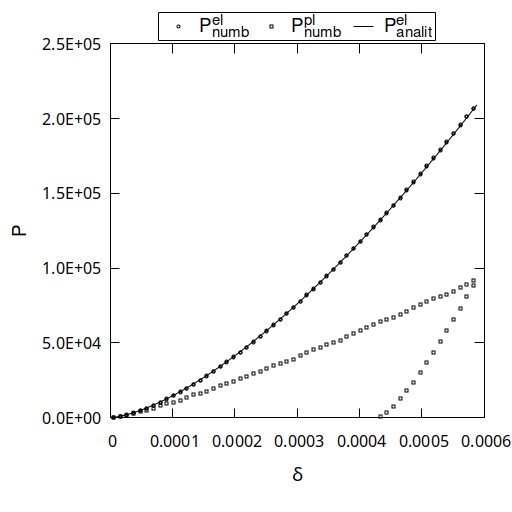
\includegraphics[height=0.3\textheight]{pictures/P_d.png}
	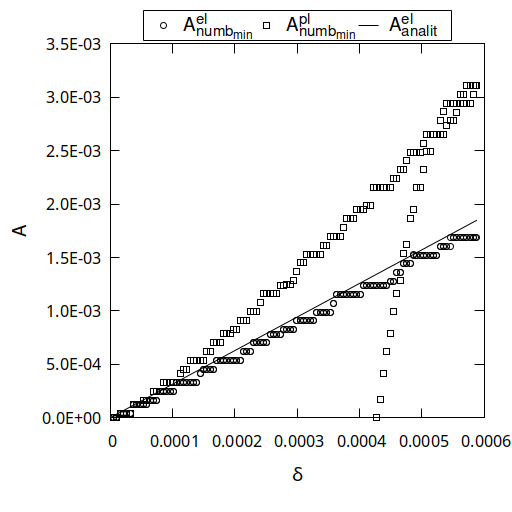
\includegraphics[height=0.3\textheight]{pictures/A_d.png}
	\caption{Решение}
	\label{fig:test1}
\end{figure}

\newpage
\section{Тест: контакт и пластичности в плосконапряжённом случае}
\begin{figure}[!h]
	\centering
	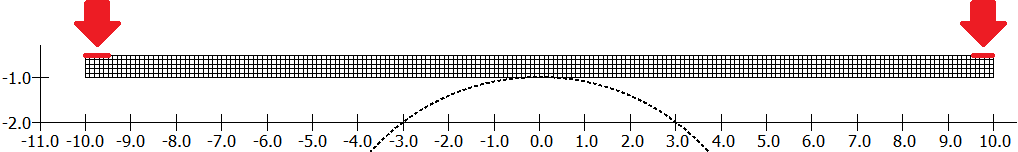
\includegraphics[height=0.08\textheight]{pictures/contact_test.png}
	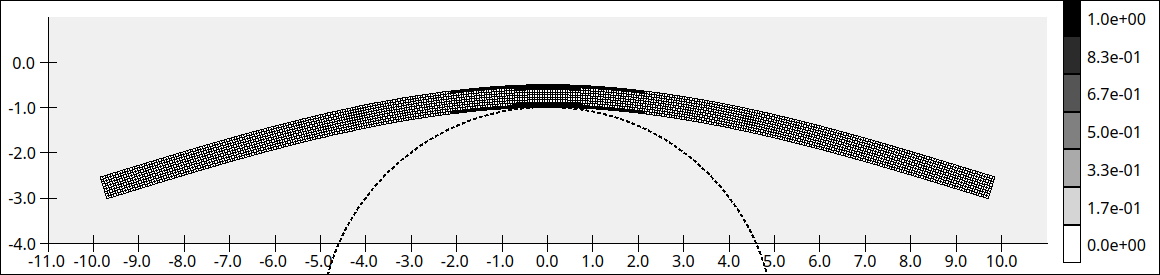
\includegraphics[height=0.13\textheight]{pictures/0.png}
	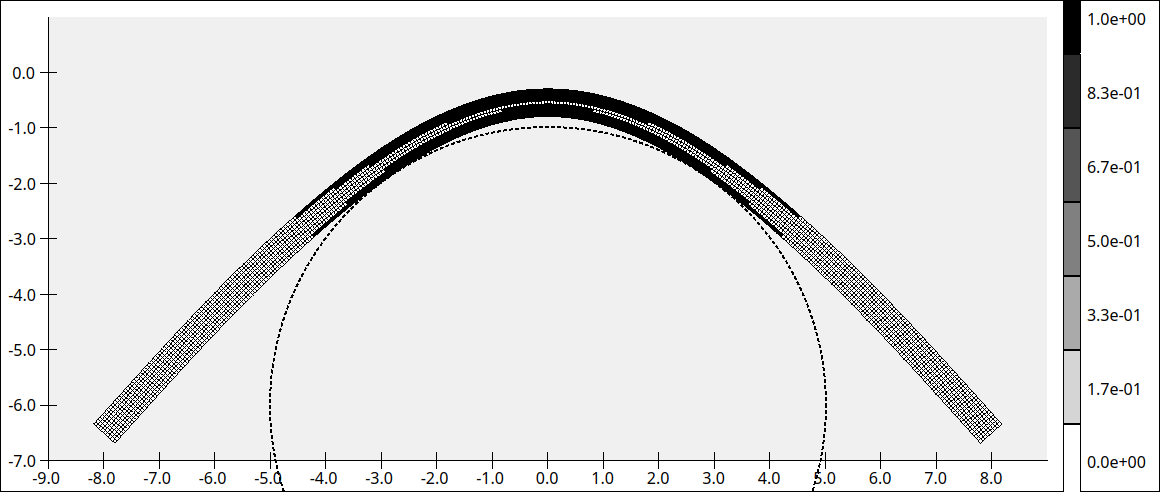
\includegraphics[height=0.2\textheight]{pictures/1.png}
	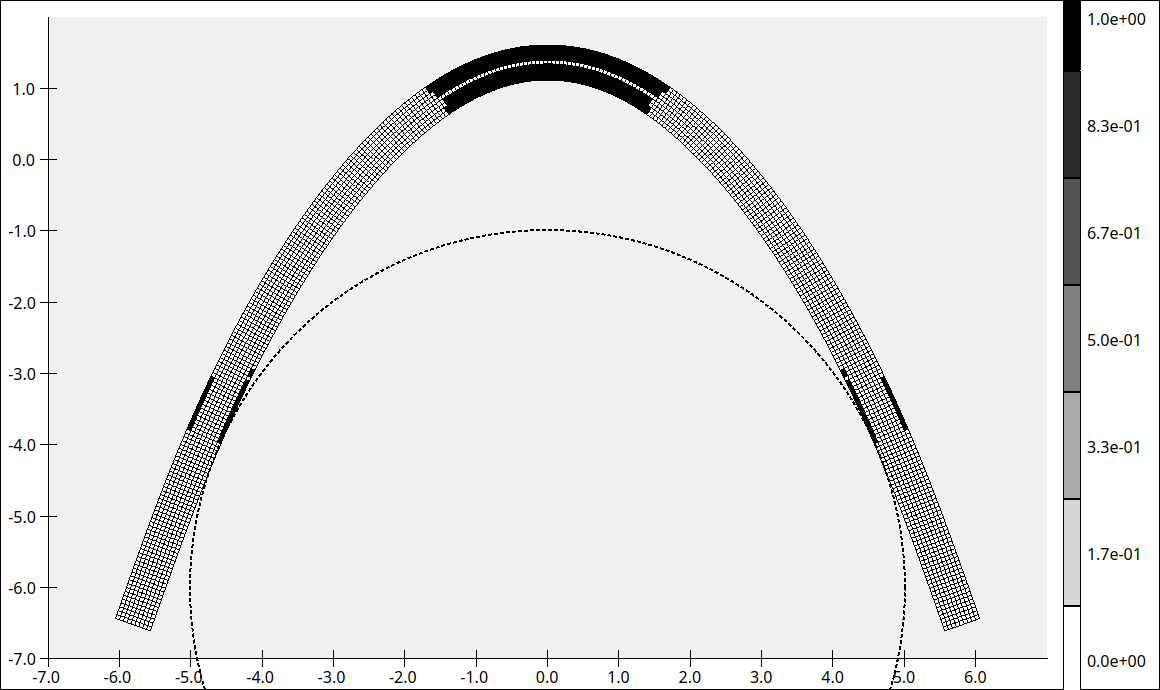
\includegraphics[height=0.2\textheight]{pictures/2.png}
	
	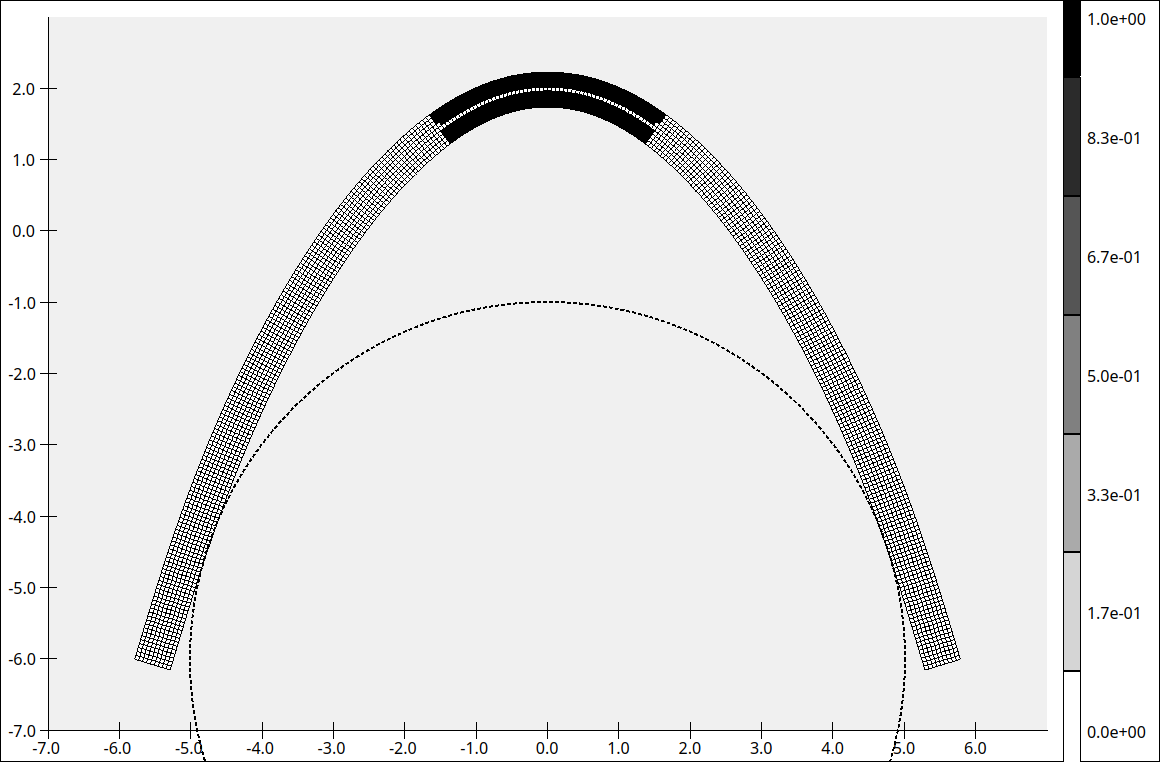
\includegraphics[height=0.2\textheight]{pictures/3.png}
	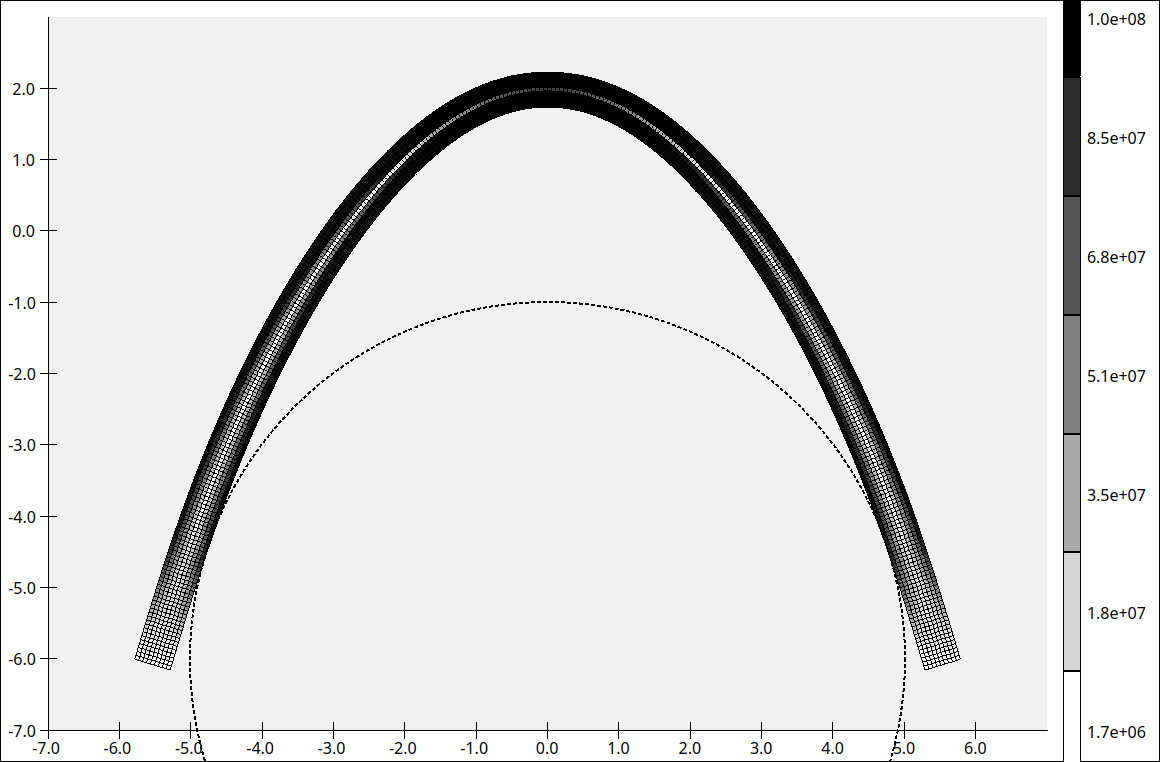
\includegraphics[height=0.2\textheight]{pictures/3_eqv.png}
	\caption{процесс нагружения}
	\label{fig:test0}
\end{figure}
Один из узлов изначально задан контактным. $\omega^{\mathrm{mp}}=1$; 50 шагов; без упрочнения.

\section{Учёт ползучести}
В соответствии с наследственной теорией ползучести, величина деформации ползучести при одноосном нагружении определяется выражением \cite{Radchenko2005}
\begin{equation}
\varepsilon^{c}=\int\limits_0^t K\left(t-\tau\right) \sigma\left(\tau \right)d\tau.
\label{F:F_creep_1d}
\end{equation}

В трёхмерном случае по теории течения
\begin{equation}
\begin{gathered}
{}^{(t)}\tilde{\varepsilon}^{c}=\int\limits_0^t K\left(t-\tau\right) \tilde{\sigma}\left(\tau \right)d\tau,\\
\Delta\tilde{\varepsilon}^{c}=\int\limits_0^{t} \left( K\left(t+\Delta t-\tau\right)-K\left(t-\tau\right)\right)  \tilde{\sigma}\left(\tau \right)d\tau+\\
+\int\limits_t^{t+\Delta t} K\left(t+\Delta t-\tau\right) \tilde{\sigma}\left(\tau \right)d\tau.
\label{F:F_creep_3d}
\end{gathered}
\end{equation}

Вместе с пластичностью \eqref{F:F_alg_ce_main}
\begin{equation}
\begin{gathered}
\Delta\sigma=\tilde{C}:\Delta\varepsilon-C:\Delta\varepsilon^{\mathrm{th}}+\Delta\sigma^{0}+\Delta\sigma^{c},\\
\Delta\sigma^{c}=-\frac{1}{2\mu}\Delta\tilde{\varepsilon}^{c}\,h_{k},
\end{gathered}
\label{F:F_creep_ce}
\end{equation}
где $\Delta\tilde{\varepsilon}^{c}$ нелинейно зависит как минимум от ${}^{(t+\Delta t)}\tilde{\sigma}$. Пластические деформации добавляются если происходит превышение предела текучести с параметром упрочнения
\begin{equation}
q=\int d\tilde{\varepsilon}^{p}+\int d\tilde{\varepsilon}^{c}.
\label{F:F_creep_Odquist}
\end{equation}

Примеры ядра ползучести \cite{Zarubin2005} (с особенностью и без):
\begin{equation}
\begin{gathered}
K=\frac{a_1+a_2\left(t-\tau\right)+a_3 T+a_4 J_2}{\left(t-\tau\right)^{\alpha}},\\
K=\frac{a_1+a_2\left(t-\tau\right)+a_3 T+a_4 J_2}{\mathrm{exp}\left(\alpha\left(t-\tau\right)\right)},
\end{gathered}
\label{F:F_creep_core}
\end{equation}
где $J_2=-\frac{1}{2}s:s$ --- второй инвариант тензора напряжений

\section{Метод Ньютона-Рафсона-Канторовича}
На шаге по времени уравнение
\begin{equation}
\mathbf{G}\left(\mathbf{q}\right)\;\mathbf{q}=\mathbf{b}\left(\mathbf{q}\right)
\end{equation}
решается по формуле (?)
\begin{equation}
\mathbf{G}\left(\mathbf{q}_k\right)\;\left(\mathbf{q}_{k+1}-\mathbf{q}_{k}\right)=
\mathbf{b}\left(\mathbf{q}_k\right)%-\mathbf{G}\left(\mathbf{q}_k\right)\;\mathbf{q}_k
\end{equation}
где матрица $\mathbf{G}\left(\mathbf{q}_k\right)$ строится с касательными тензорами $\tilde{C}=\frac{\partial\sigma\left(\mathbf{q}_k\right) }{\partial\varepsilon}$. Вектор $\mathbf{b}\left(\mathbf{q}_k\right)$ включает невязку между силами и внутренними напряжениями. Матрица $\mathbf{G}\left(\mathbf{q}_k\right)$ и вектор $\mathbf{b}\left(\mathbf{q}_k\right)$ строятся на сдвинутой перемещениями $\mathbf{q}_k$ сетке. Можно записать
\begin{equation}
\mathbf{q}_{k+1}=\mathbf{q}_{k}+\mathbf{G}^{-1}\left(\mathbf{q}_k\right)\;\mathbf{b}\left(\mathbf{q}_k\right)
%\mathbf{q}_{k+1}=\mathbf{q}_{k}+\mathbf{G}^{-1}\left(\mathbf{q}_k\right)\;\left(\mathbf{b}\left(\mathbf{q}_k\right)-\mathbf{G}\left(\mathbf{q}_k\right)\;\mathbf{q}_k\right) 
\end{equation}
\section{Большие деформации}
Выбор объективных тензоров деформаций и напряжений, и их производных зависит от определяющих соотношений \cite{Korobeynikov2000}
\section{Оптимизация}
Есть в \cite{Smetannikov2009,Bormotin2019}
\chapter{Заключение}
%\section{Заключение}
Составлены и реализованы эффективные и хорошо сходящиеся при сложном нагружении численные схемы для решения контактных задач с физической нелинейностью на основе теории течения.
\begin{thebibliography}{3}
	\bibitem{Pisarenko1981}
	Писаренко Г. С., Можаровский Н. С. Уравнения и краевые задачи теории пластичности и ползучести. --- Киев : Наукова думка, 1981. --- 496 с.
	\bibitem{Kravchuk1994}
	Кравчук А. С. Вариационные и квазивариационные неравенства в механике. --- РФФИ, 1994. --- 334 с.
	\bibitem{Korobeynikov2000}
	Коробейников С. Н. Нелинейное деформирование твердых тел. --- Новосибирск : Издательство СО РАН, 2000. --- 262 с.
	\bibitem{SoloveychikRoyakPersova2007}
	Соловейчик Ю. Г., Рояк М. Э., Персова М. Г. Метод конечных элементов для решения скалярных и векторных задач. --- Новосибирск : Изд-­во НГТУ, 2007. --- 895 с.
	\bibitem{Zienkiewicz1975}
	Зенкевич О. Метод конечных элементов в технике. --- М. : Мир, 1975. --- 542 с.
	\bibitem{Frolov1995}
	Александров А. В., Алфутов Н. А., Астанин В. В. и др. Энциклопедия ”Машиностроение”. Том I-­3. ”Динамика и прочность машин. Теория механизмов и машин”. В 2-­х книгах. Кн. 2 / Под ред. Фролов К. В. (гл. ред.). --- М. : Машиностроение, 1995. --- 624 с.
	\bibitem{Belytschko2000}
	Belytschko T., Liu W. K., Moran B. Nonlinear finite elements for continua and structures, 2000.
	%\bibitem{OtchetPNI}
	%Отчет о ПНИ по теме: "Разработка программно-технических решений в области промышленного программного обеспечения для моделирования поведения элементов конструкций из современных материалов в экстремальных условиях при механических и немеханических воздействиях для решения задач проектирования авиакосмической техники" (No гос. регистрации: 114112440083)
	\bibitem{Ortiz1985}
	Ortiz M., Popov E. P. Accuracy and stability of integration algorithms for elastoplastic constitutive relations //International journal for numerical methods in engineering. – 1985. – Т. 21. – №. 9. – С. 1561-1576.
	\bibitem{Wriggers2006}
	Wriggers P. Computational Contact Mechanics. --- Springer Science \& Business Media, 2006.
	\bibitem{Radchenko2005}
	Радченко В. П., Саушкин М. Н. Ползучесть и релаксация остаточных напряжений в упрочнённых конструкциях. – Mikhail Saushkin, 2005.
	\bibitem{Zarubin2005}
	Зарубин В. С., Станкевич И. В. Расчет теплонапряженных конструкций. – 2005.
	\bibitem{Smetannikov2009}
	Матвеенко В. П. и др. Термомеханика полимерных материалов в условиях релаксационного перехода. – 2009.
	\bibitem{Bormotin2019}
	Бормотин К. С., Вин А. Численный метод оптимизации процесса формообразования панелей обтяжкой //вычислительные методы и программирование. – 2019. – Т. 20. – С. 386-395.
	
\end{thebibliography}





%%% Local Variables:
%%% mode: latex
%%% TeX-master: "rpz"
%%% End:
